\documentclass{beamer}

\usepackage[utf8]{inputenc} % Ensure proper encoding
\usepackage{graphicx} % For including images
\usepackage{hyperref} % For hyperlinks
\usepackage{amsmath,amsfonts,amssymb} % For mathematical symbols and equations
\begin{document}

\title{Workfare versus Welfare: Incentive Arguments for Work Requirements in PovertyAlleviation Programs}
\author{Timothy Besley \& Stephen Coate}
\date{\today}

\frame{\titlepage}


\begin{frame}
\frametitle{Introduction}
\begin{itemize}
\item How should govt design poverty alleviation programs? 
\item Should these programs require a work condition or not?
\item Work requirements provide incentives to earn. Two potential incentives arguments are :
\begin{itemize}
    \item A screening argument that work requirements may serve as a means of targeting transfer.
    \item A deterrent argument that they may serve as a device to encourage poverty-reducing investments
\end{itemize}
\end{itemize}
\end{frame}

\begin{frame}
\frametitle{Screening Argument }
\begin{itemize}
    \item It is very costly to set up a proxy means testing type rule to target poor. It is particularly costly for developing countries that lack the administrative capacity and data.
    \item In such situations, it may be better to make the relief system self-targeting by laying down conditions for claiming support such that only the truly needy present themselves.
    \item Even in developing countries, you might observe the earned income but the potential earnings and therefore there remains an argument for screening through workfare. 
  
\end{itemize}
\end{frame}

\begin{frame}{Deterrence Argument}
\begin{itemize}
    \item This relies on the question whether people are poor by choice i.e, they do not want to work or because of bad luck i.e, they could not find work. 
    \item In case of latter, public assistance can distort incentives (such as divorce if single parents get more benefits). 
    \item Therefore public assistance should be made less attractive by creating some deterrence. 
\end{itemize}
\end{frame}

\begin{frame}{Baseline Poverty Alleviation Program (PAP) with perfect information}
\begin{itemize}
    \item We consider a population consisting of n
 individuals, divided into two types according
 to their income-generating ability or wages, $ a \in
 \{a_L, a_H\},$ where $a_L <a_H $ and where H stands
 for high and L stands for low. A fraction $\gamma$
 has ability $a_L$. Each individual has identical quasi-linear preferences defined over income y and work l. Thus, utility is given by y - h(l) where
 h(.) is increasing and strictly convex.
 \item A PAP is pair of benefits and costs $\{b_i , c_i\}$. $b_i$ is benefit for individual of type i and $c_i$ is the cost. 
 \item The to govt is $n \gamma b_L + n(1-\gamma) b_H$
 \item The govt objective is to minimize cost and ensure each individual gets at least z dollars. 
 \item Both types of individuals choose whether to claim benefits.
\end{itemize}

\end{frame}

\begin{frame}{PAP Continued }
\begin{itemize}
    \item The private sector labor supply if individual accepts the program is 
    \[l(b,c,a_i )= \case \]
\end{itemize}
\end{frame}

\begin{frame}{RMTR}
\begin{figure}
    \centering
    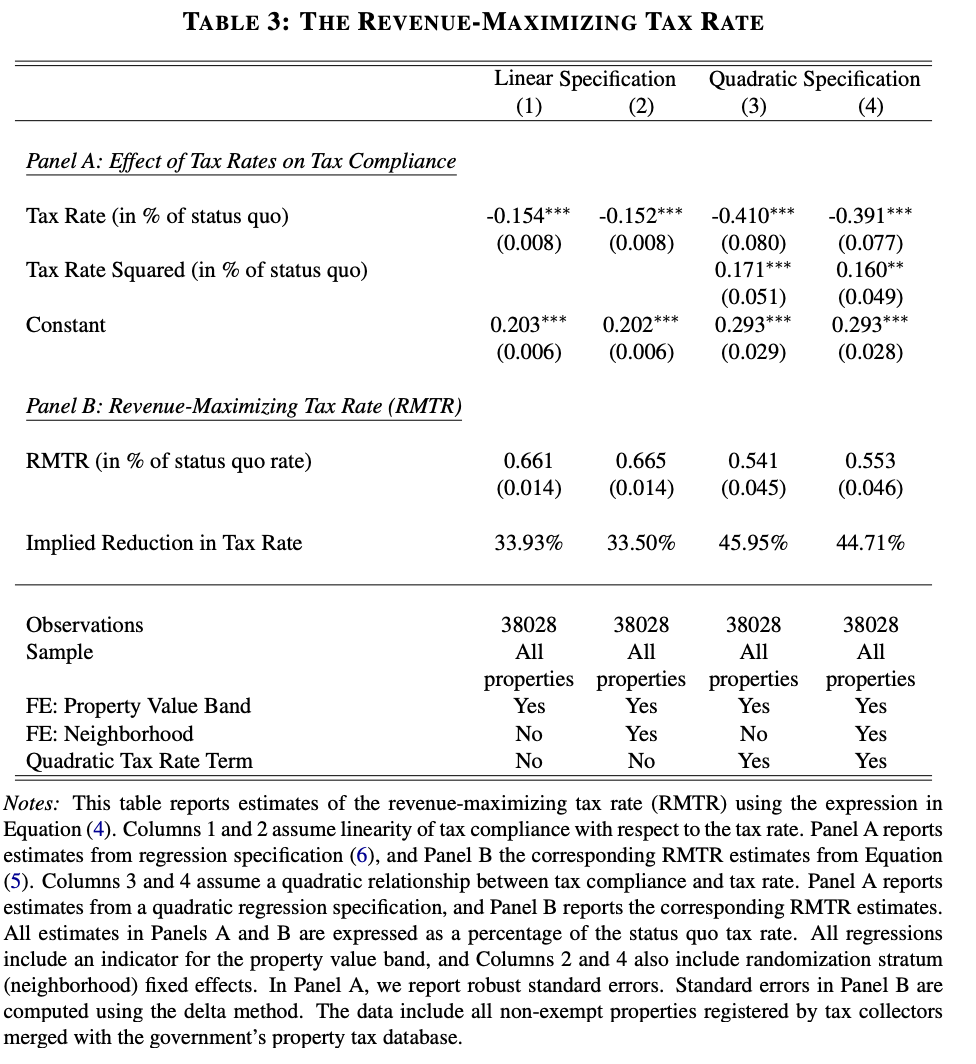
\includegraphics[width=\textwidth,height=0.8\textheight]{Paper Presentations/The State Capacity Ceiling on Tax Rates/T3.png}
    \label{fig:enter-label}
\end{figure}
\end{frame}

\begin{frame}{RMTR and Enforcement}
\begin{figure}
    \centering
    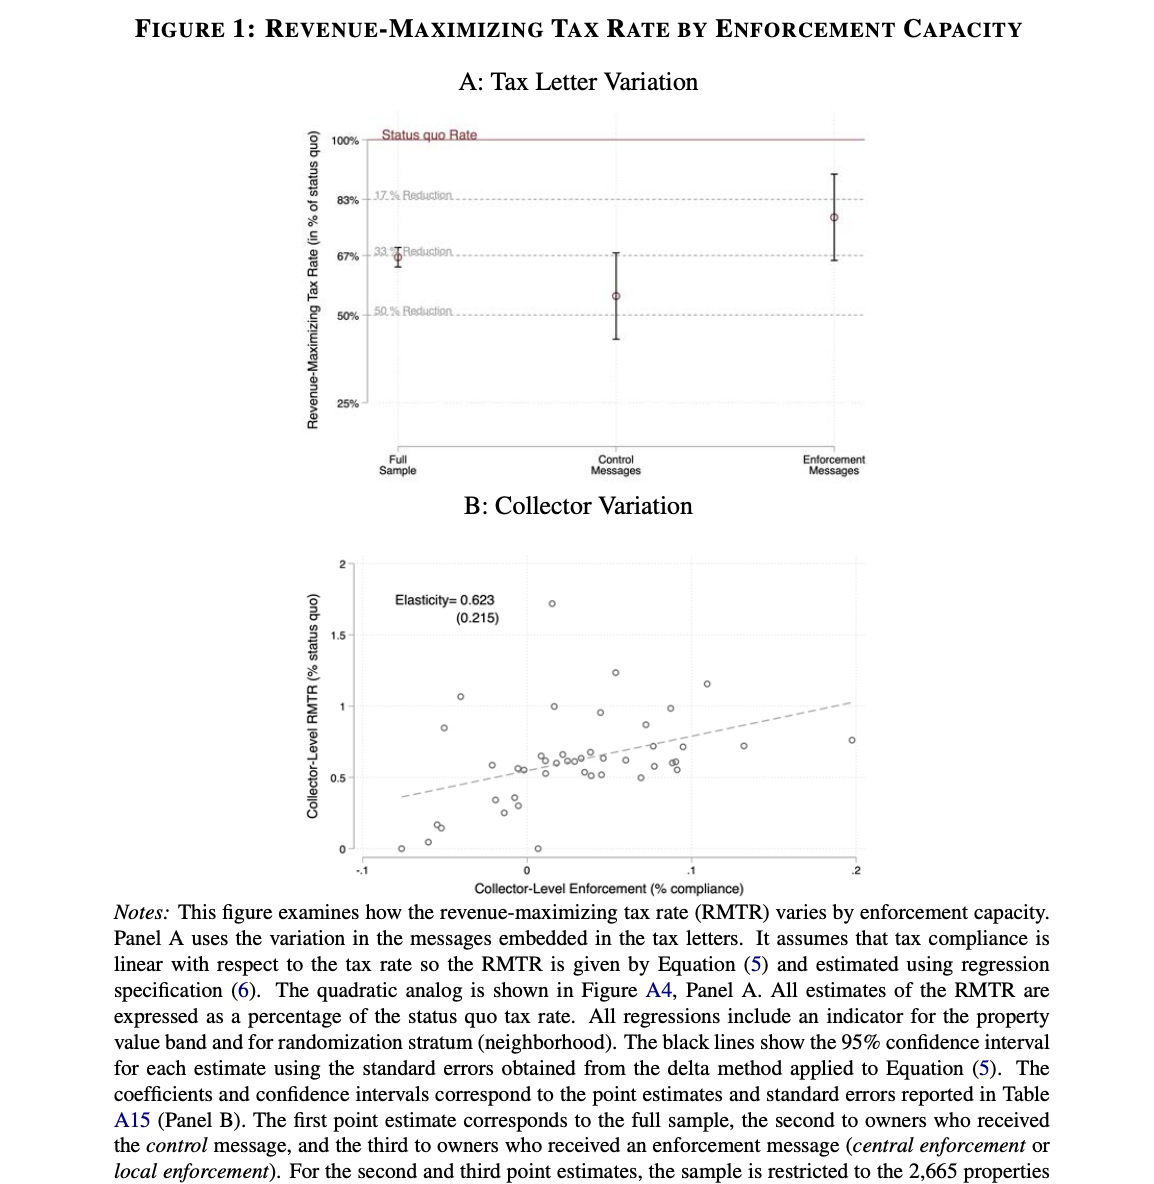
\includegraphics[height=\textheight,width=\textwidth]{Paper Presentations/The State Capacity Ceiling on Tax Rates/F1.png}
    \label{fig:enter-label}
\end{figure}
\end{frame}



\begin{frame}
\frametitle{Rates and Enforcement as Complements}
\begin{figure}
    \centering
    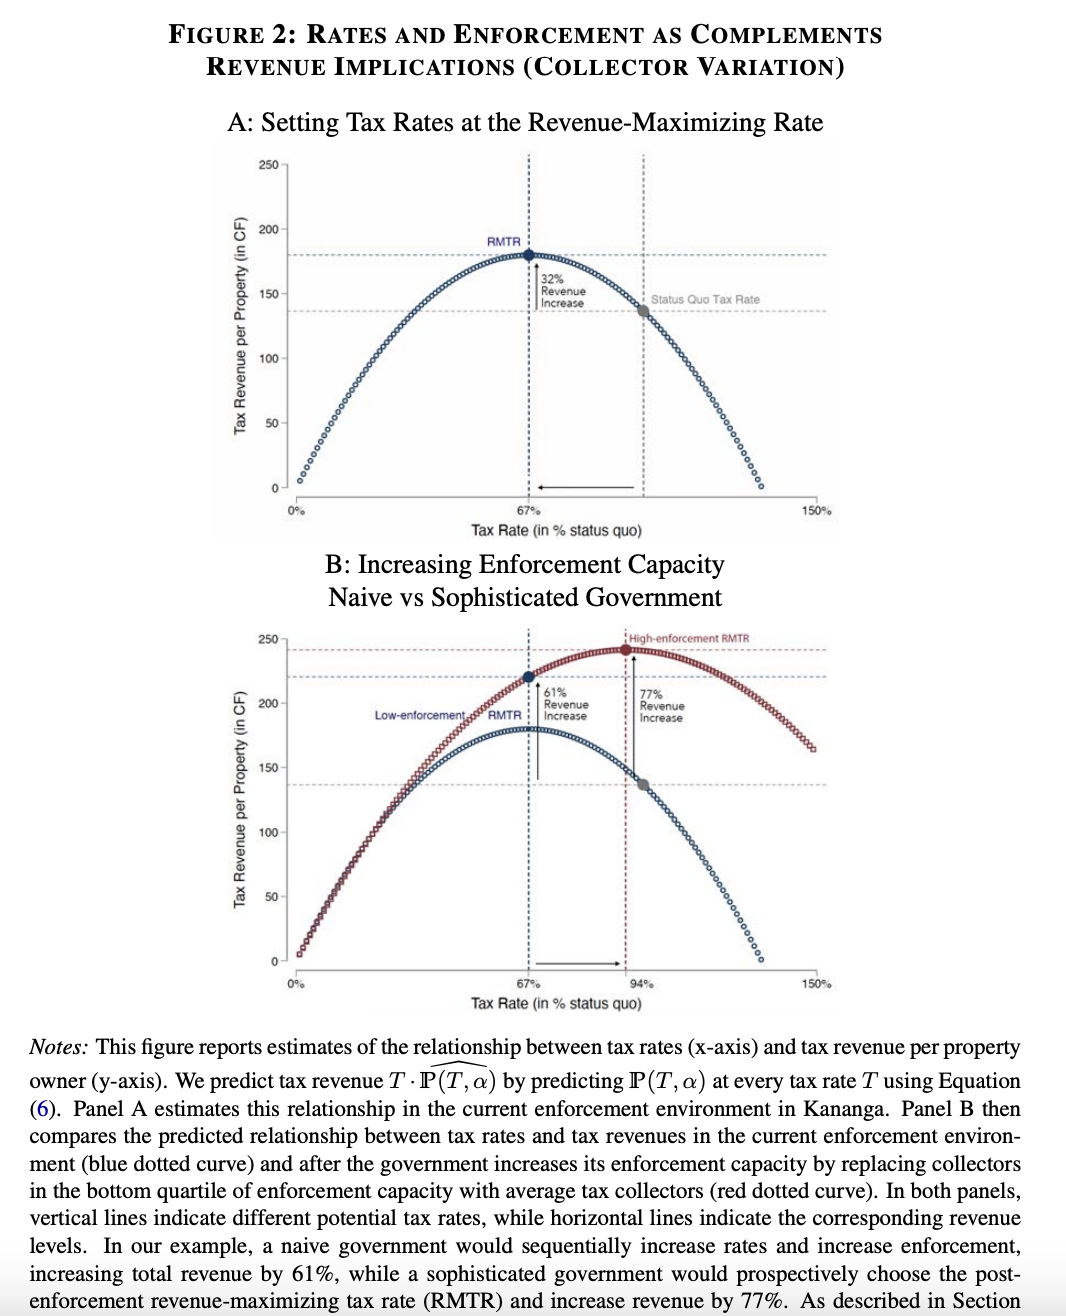
\includegraphics[height=0.9\textheight,width=\textwidth]{Paper Presentations/The State Capacity Ceiling on Tax Rates/F2.png}
\end{figure}
\end{frame}

\begin{frame}{Questions}
    \begin{itemize}
        \item Does it mean that when tax rate is lower, it is not optimal for taxpayers to evade it and therefore they pay it?
        \item Does it mean governments with weak state capacity should start with very low tax rates?
        \item What does this mean for other taxes, in particular taxation of businesses?
        \item It is very important to think about this question in public finance that when govt has very low capacity and they want to start raising revenue to build the capacity, what are lessons there?
    \end{itemize}
\end{frame}
\begin{frame}
\frametitle{Conclusions}
\begin{itemize}
\item Tax rates and enforcement are thus complementary levers. 
\item Jointly optimizing tax rates and
enforcement would lead to 26\% higher revenue gains than optimizing them independently.
\item These
findings provide experimental evidence that low government enforcement capacity sets a binding
ceiling on the revenue-maximizing tax rate in some developing countries, thereby demonstrating
the value of increasing tax rates in tandem with enforcement to expand fiscal capacity
\end{itemize}
\end{frame}

\end{document}

\begin{frame}
  \titlepage
\end{frame}



\end{document}
